\begin{figure}
	\centering
	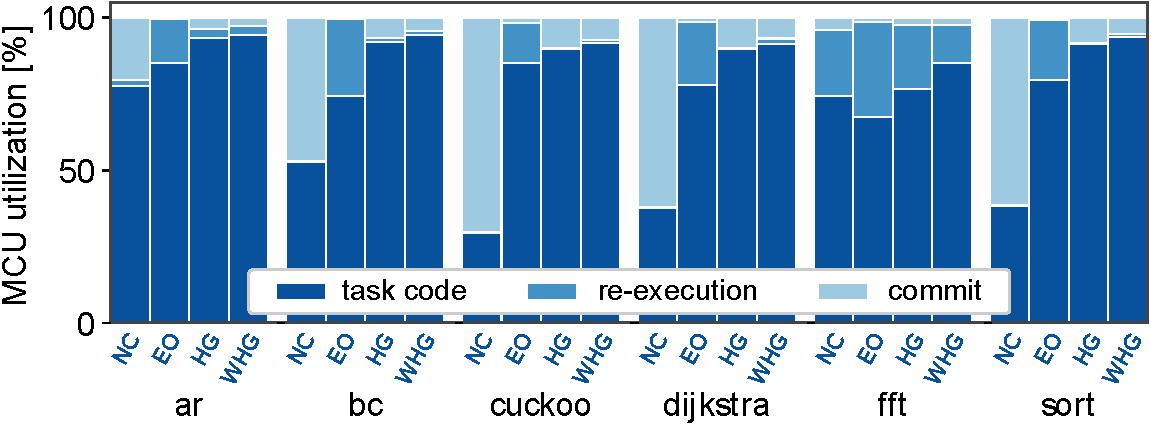
\includegraphics[width=\columnwidth]{figures/coalEfficiency}
    \caption{Breakdown of overhead for the proposed coalescing strategies.
NC: no coalescing, EO: energy-oblivious coalescing, EG: Energy-guided coalescing, WEG:
energy- and task-aware coalescing. All coalescing strategies reduce total
overhead and maximize useful work. EG and WEG perform better than EO.}
	\label{fig:overallOverheadBreakdown}
\end{figure}
% \end{wrapfigure}
%
%Building on top of the existing work, we have selected the most efficient task-based run-time library~\cite{alpaca} and compared \sys against it.
Our evaluation quantitatively demonstrates that \sys (i) \emph{reduces the memory
protection overhead} by coalescing, (ii) \emph{improves execution speed}, in most cases; %
and (iii) \sys is able to progress where static systems suffer from a task non-termination loop. 
We have also broken down \sys's overhead to explain the source of \sys's improved performance.
%
\subsection{Characterization of Overhead}
\label{sec:coala_overhead}

\subsubsection{Overhead Reduced by Coalescing}
\label{sec:overhead-coalescing}

For each coalescing strategy from Section~\ref{sec:task_adaptation} (EO, EG,
and WEG) and for a baseline without coalescing (NC), we have measured the time
spent on (i) executing task code (ii) re-executing task code after a power failure, and
(iii) committing state to non-volatile memory at the end of each (coalesced)
task.  In this experiment the WISP was 15\,cm away from the signal generator
antenna.

The overhead incurred by each coalescing strategy is broken down in
Fig.~\ref{fig:overallOverheadBreakdown}. Without coalescing enabled (NC), the
re-execution penalty is smallest, because the amount of work that can happen
between commits and may have to be re-executed if interrupted is smallest when
work from multiple static tasks is not combined.
%
However, any gain from a reduced re-execution penalty is canceled out by
the increased commit overhead that is incurred at the end of each static
task.
%
Across all benchmarks, all coalescing strategies reduce more commit overhead
than the re-execution overhead they add.
%
This net overhead reduction is greatest in EG and WEG strategies compared
to the EO strategy. We attribute this discrepancy to EO's slow adjustment
of the target task size without regard to the energy conditions.
%
In the subsequent experiments, we focus on the better-performing EG and WEG
strategies.
%
\begin{figure}
	\centering
	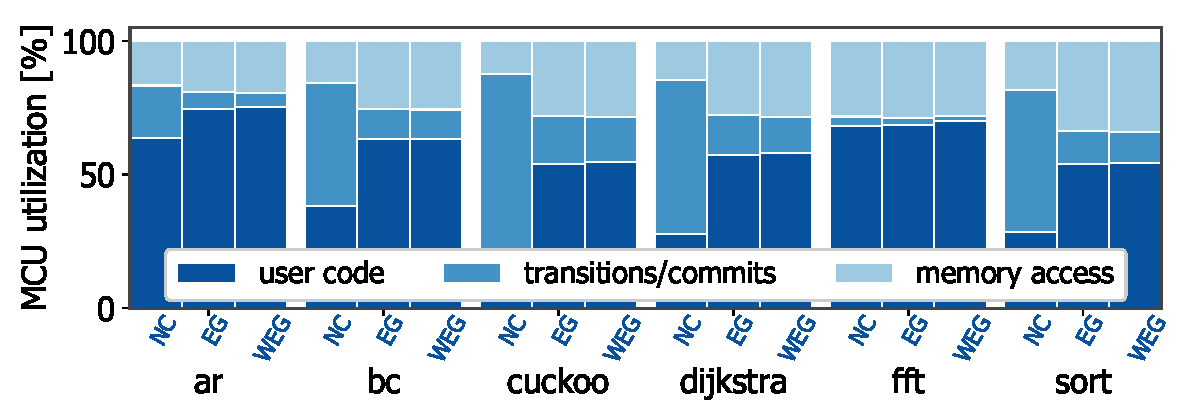
\includegraphics[width=\columnwidth]{figures/overallOverhead}
	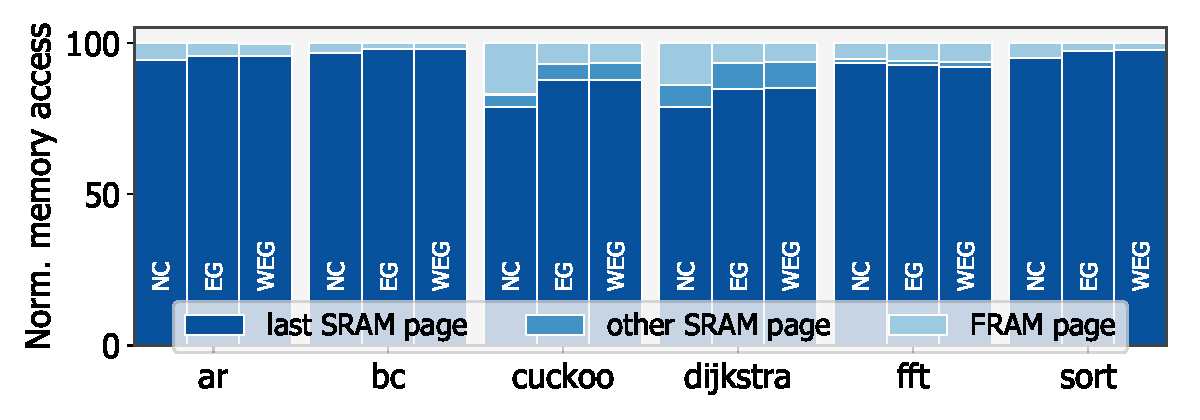
\includegraphics[width=\columnwidth]{figures/memAccess}
	\caption{\sys kernel overhead: a breakdown of time spent in
the application and in the runtime (top) and a breakdown of protected memory
accesses into three types with different costs. NC: no coalescing, EG:
Energy-guided coalescing, WEG: weighted Energy-guided coalescing.}
	\label{fig:coalEfficiency}
\end{figure}
%
\subsubsection{\sys Kernel Overhead Breakdown}
%
Fig.~\ref{fig:coalEfficiency} (top) breaks down the time spent on executing 
task code and committing further into time spent by the application and
time spent by \sys's runtime. When coalescing is not enabled the commit overhead is 
highest.
%
However, coalescing increases the cost of each access to a protected variable,
since VMM has to spend more on average time in searching for the requested page.
%
For both coalescing strategies (EG and WEG) accesses to protected variables
constitute about 30\% of the runtime overhead. Dynamic address translation
necessary on each protected access is the most critical bottleneck for \sys.
%
\subsubsection{Protected Memory Accesses Breakdown}
%
Fig.~\ref{fig:coalEfficiency} (bottom) breaks down protected memory accesses
into three categories.
%
Each type of protected access incurs a different amount of overhead: access to
the same page in SRAM as the previous access is cheapest, access to a different
SRAM page has a larger cost, and access to a page that needs to be swapped in
from FRAM into SRAM is most expensive.
%
The results in the figure show that the overwhelming majority of accesses are
of the cheapest kind, which motivated us to optimize this access type in our
implementation (see Section~\ref{sec:impl:paging}).
%
Only \textit{cuckoo}, \textit{dijkstra}, and \textit{fft} have non-negligible
number of accesses to a different SRAM page, which is due to the larger working
set and a less regular access pattern in these applications.
%
In general, memory access patterns are shaped by the application, and the more
program state is protected, the higher the rate of page swaps.
%
\subsection{Execution time}
\label{sec:result_coalescing}
%
Having shown in Section~\ref{sec:coala_overhead} that coalescing reduces
overhead, we now investigate the outcome of this reduction on the total
execution time. We first investigate difference variants of \sys and
then compare the best variant to Alpaca~\cite{alpaca}.
%
\subsubsection{\sys Speedup with Coalescing}

Fig.~\ref{fig:coalescing} shows the \sys run time with two coalescing
strategies (EG, WEG) normalized to the run time without coalescing (NC).
%
The results in Fig.~\ref{fig:coalescing} show that all benchmarks
complete faster with coalescing than without coalescing: from 25\% faster
(\textit{ar}) up to 70\% faster (\textit{sort}).
%
This speedup is a consequence of the reduced overhead demonstrated in
Section~\ref{sec:coala_overhead}.
%
However, the magnitude of the speedup is (1) highly application-dependent and
(2) largely similar across the two coalescing strategies, with the exception of
\textit{fft}.
%
In some cases (\textit{bc}, \textit{cuckoo}, \textit{sort}) the Weight Energy-guided
feature in the coalescing algorithm is counter-productive.
%
This occurs in task decompositions with a uniform task energy, where counting
tasks disregarding their energy provides an equal amount of information with a
smaller effort.
%
In \textit{fft}, tasks are not uniform, and accounting for task energies is
beneficial. In fact, the lack of task energy awareness is detrimental: with EG
\textit{fft} runs slower than without any coalescing (NC).
%
The speedup is highest for \textit{bc}, \textit{cuckoo}, \textit{dijkstra} and
\textit{sort}, because their tasks are relatively small and are easily coalesced,
eliminating many unnecessary commits.
%
\begin{figure}
	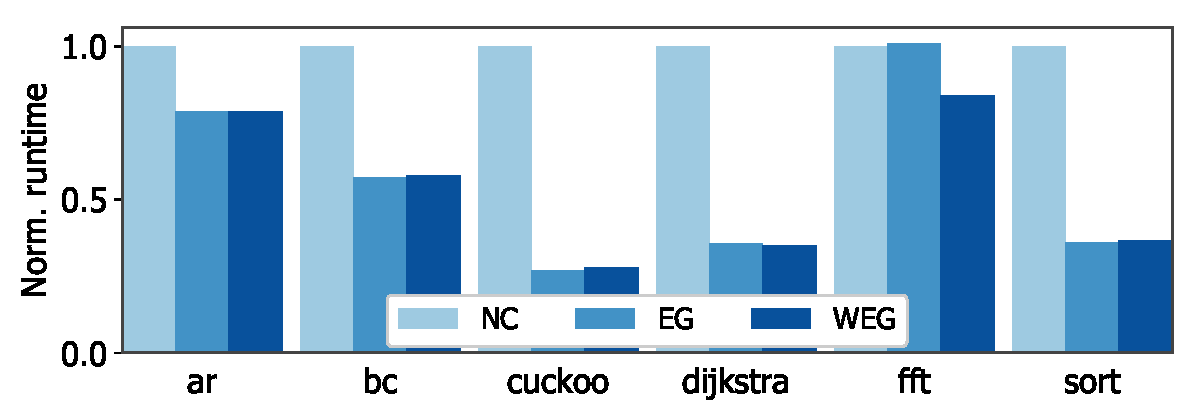
\includegraphics[width=\columnwidth]{figures/coalStrategies}%
    \caption{\sys's coalescing performance.  Application execution time
with coalescing strategies (EG and WEG) normalized to the execution time
without coalescing.}
	\label{fig:coalescing}
\end{figure}

\begin{figure}
	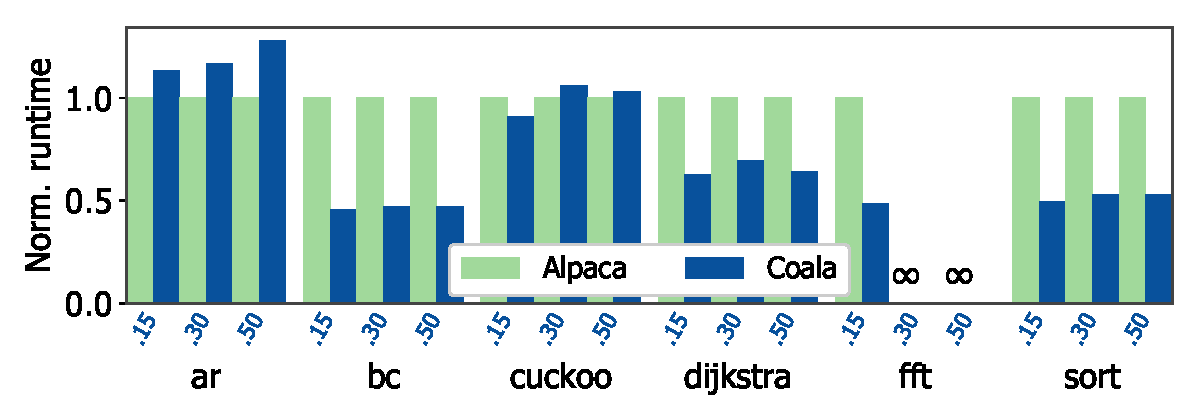
\includegraphics[width=\columnwidth]{figures/coala_alpaca_gcc}
    \caption{\sys's execution time, normalized, where possible, to the execution time 
    with Alpaca, as a function of distance to the energy source 
    measured in meter.}
	\label{fig:runtime}
\end{figure}

\subsubsection{Benefits of Adaptive Tasks}
%
We now compare \sys's performance to Alpaca~\cite{alpaca}---a
\emph{non-adaptive} task-based system with tasks fixed at compile time.
Fig.~\ref{fig:runtime} shows the average execution time of each
application for \sys and Alpaca, normalized, where possible, to the latter. The results show
that \sys provides a performance benefit compared to Alpaca for most
applications. The speedup is greatest for applications with repeated write after
read dependencies throughout their code, particularly involving arrays
(\textit{dijkstra}, \textit{fft} and \textit{sort}). \sys's VMM
successfully amortizes the overhead of protecting memory that is accessed in
such patterns.  In applications without locality among accesses to protected
variables, including array elements, \sys incurs overhead from memory
virtualization that causes its performance to be comparable to (or worse than)
Alpaca (\textit{ar}, \textit{cuckoo}).

Due to its static progressing behavior Alpaca was unable to finish the \textit{fft} benchmark on a distance larger than 15\,cm\footnote{At distances greater than 15\,cm, energy incoming during
execution is negligible and stored energy is insufficient to complete some of
the static tasks.}. This is marked with $\infty$ signs in Fig.~\ref{fig:coalescing}. \sys, however, manged to complete \textit{fft} application by enabling its task downscaling on the distances 30\,cm and 50\,cm.
 
Overall, \sys shows better performance than its counterpart, and it is able to overcome the \textit{big task} (i.e. \textit{fft} tasks) problem that the static task-based systems suffer from. 

\subsection{Virtual Memory Performance}
\label{sec:results_memory_management}

We characterize the performance of \sys's virtual memory sub-system in an
experiment on a continuously-powered evaluation board described in
Section~\ref{sec:methodology}.  Fig.~\ref{fig:page_size} quantifies the
effects of page size.
%
\begin{figure}
	\centering
	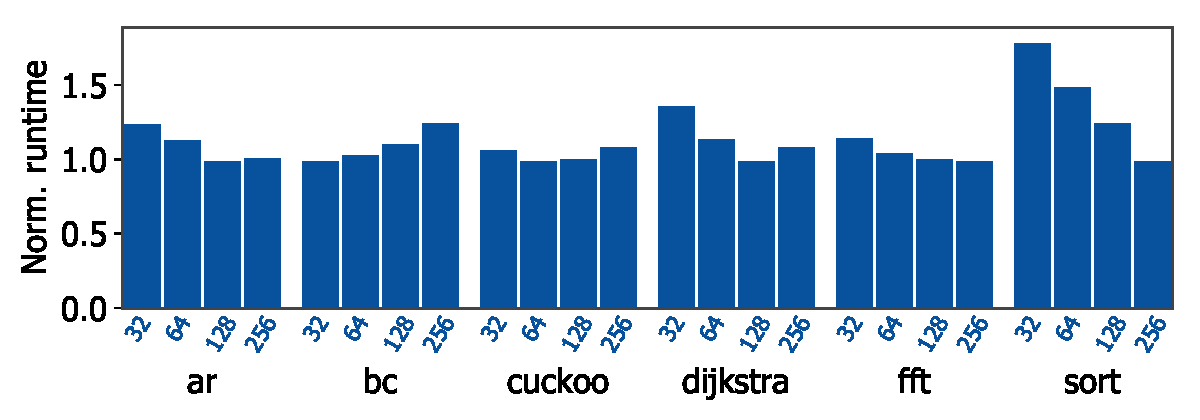
\includegraphics[width=\columnwidth]{figures/page_exec-time}
	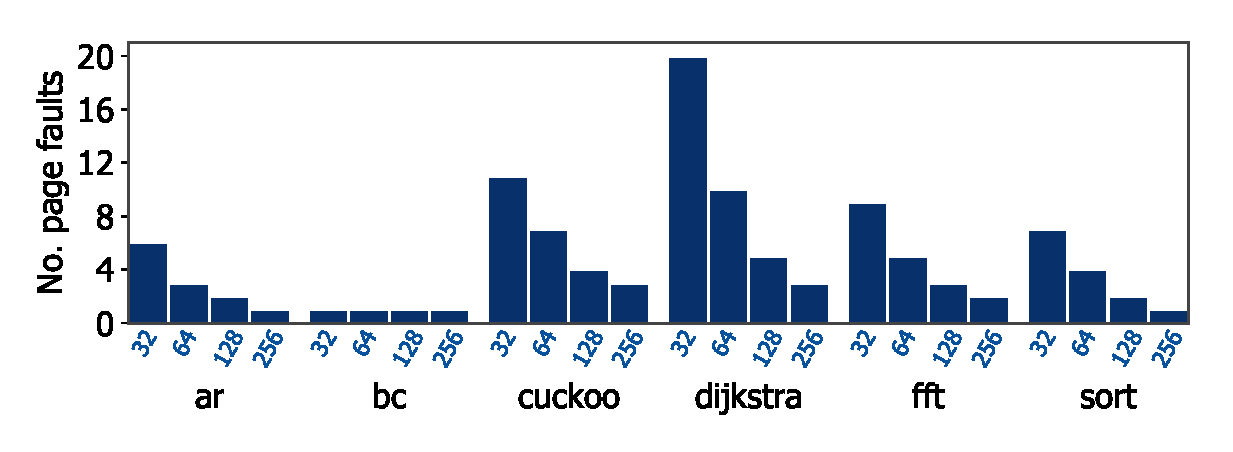
\includegraphics[width=\columnwidth]{figures/pagePulls}
    \caption{Effect of page size on execution time (top) and on the number of
page faults (bottom). The execution time is normalized to the lowest in each set
of page sizes.}
	\label{fig:page_size}
\end{figure}
%
\subsubsection{Effect of Page Size on Runtime}
%
Fig.~\ref{fig:page_size} (top) shows the execution time as a function
of page size, normalized to the lowest per-application performance among the
set of page sizes.
The data suggest that there is a page size, distinct from the largest or
smallest, that minimizes execution time. The best page size is not the same for
each application. Nevertheless, if a choice must be made for all applications,
128\,B pages perform well for most of them.
%
\subsubsection{Effect of Page Size on Page Faults}
%
Fig.~\ref{fig:page_size} (bottom) shows the number of page faults as a
function of page size.
%
The smaller the page the more likely that a memory access will land
outside that page and that a new page will need to be swapped in.
%
This trend is visible for all applications, exception \textit{bc}. The total
amount of data accessed by \textit{bc}, as well as its working set, is small.
Even with the smallest page, all accesses are contained within that page, and
no page faults occur. Without any page faults to begin with, increasing the
page size result only in overhead.